% -*- root: main.tex -*-

\chapter{Loose ends}

\todo[inline]{I'd like to spend a couple of days talking about ways the picture in this class can be extended, finally, some actually unanswered questions that naturally arise.  The following two section titles are totally made up and probably won't last.}
\todo[inline]{Also, write a broad-scale introduction to this appendix.}







\section{Orientations by \texorpdfstring{$E_\infty$}{Eoo} maps}

A more modern take on the story of the $\sigma$--orientation passes through the algebraic geometry of $E_\infty$--ring spectra, which are the homotopically coherent analogues of commutative ring objects that one finds in the $\infty$--category $\CatOf{Spectra}$.  Our reward for grappling with this will be the modularity of the $\String$--orientation, enriching \Cref{WittensTheoremForBU6} to the real setting.  Essentially all of the ring spectra discussed in this book have incarnations as $E_\infty$--rings:
\begin{theorem}
\citeme{this is a mega-theorem}
\todo{This is the first mention of $\tmf$.  Give a description of $\tmf$, $\TMF$, and $\Tmf$ in terms of $\moduli{ell}$.}
The classical $K$--theories $KU$ and $KO$, the Eilenberg--Mac Lane spectra $HR$, the Morava $E$--theories $E_\Gamma$, their fixed point spectra, the Thom spectra arising from the $J$--homomorphism (including $MO$, $MSO$, $M\Spin$, $M\String$, $MU$, $MSU$, and $MU[6, \infty)$), the spectra $\TMF$, $\Tmf$, and $\tmf$ are all $E_\infty$--ring spectra.\footnote{Notably, the Morava $K$--theories are \emph{not} $E_\infty$ rings at finite heights.} \qed
\end{theorem}

A great deal of classical commutative algebra can be lifted into this new setting, including a particular functor \[\gl_1\co E_\infty\CatOf{RingSpectra} \to \CatOf{Spectra}.\]  This functor derives its name from two compatible sources: for one, its underlying infinite loopspace is the construction $GL_1$ described in \Cref{LectureThomSpectra}; and secondly, it participates in an adjunction
\begin{center}
\begin{tikzcd}[column sep=4em]
\CatOf{ConnectiveSpectra} \arrow[shift left=0.3\baselineskip, "\Susp^\infty_+ \Omega^\infty"]{r} & E_\infty\CatOf{RingSpectra} \arrow[shift left=0.3\baselineskip, "\gl_1"]{l}
\end{tikzcd}
\end{center}
analogous to the adjunction between the group of units and the group-ring constructions in classical algebra.  Its relevance to us is its participation in the theory of highly structured Thom spectra.  Let $j\co g \to \gl_1 \S$ be a map of connective spectra, begetting a map $J\co G \to \GL_1 \S$ of infinite loopspaces, where we have written $G = \Loops^\infty g$.
\begin{lemma}
\citeme{May? or ABGHR?}
The Thom spectrum of the map $BJ$ is presented by the pushout of $E_\infty$ rings\footnote{This is a kind of ``twisted group-ring'' construction.}
\begin{center}
\begin{tikzcd}
\Susp^\infty_+ \GL_1 \S \arrow["\Loops^\infty \Susp j"]{r} \arrow{d} & \Susp^\infty_+ \Loops^\infty \gl_1 \S / g \arrow{d} \\
\S \arrow{r} & MG. \qed
\end{tikzcd}
\end{center}
\end{lemma}

\begin{corollary}
\citeme{May, but also ABGHR}
There is a natural equivalence between the space of null-homotopies of the composite \[g \xrightarrow j \gl_1 \S \xrightarrow{\gl_1 \eta_R} \gl_1 R\] and the space of $E_\infty$ ring maps $MG \to R$, where $MG$ is the Thom spectrum of the stable spherical bundle classified by $J$.
\end{corollary}
\begin{proof}
Applying the mapping space functor $E_\infty(-, R)$ to the pushout diagram in the Lemma, we have a pullback diagram of mapping spaces:
\begin{center}
\begin{tikzcd}
E_\infty(\Susp^\infty_+ \GL_1 \S, R) & E_\infty(\Susp^\infty_+ \Loops^\infty \gl_1 \S / g, R) \arrow{l} \\
E_\infty(\S, R) \arrow{u} & E_\infty(MG, R) \arrow{l} \arrow{u}.
\end{tikzcd}
\end{center}
We can reidentify each of the three terms to get
\begin{center}
\begin{tikzcd}
\CatOf{Spectra}(\gl_1 \S, \gl_1 R) & \CatOf{Spectra}(\gl_1 \S / g, \gl_1 R) \arrow{l} \\
\{\gl_1 \eta_R\} \arrow{u} & E_\infty(MG, R) \arrow{l} \arrow{u},
\end{tikzcd}
\end{center}
hence $E_\infty(MG, R)$ appears as the fiber at $\gl_1 \eta_R$ of the restriction map, which coincides with the space of nullhomotopies as claimed.
\end{proof}

\begin{corollary}
\citeme{AHR}
The mapping set $E_\infty(Mj, R)$ is nonempty if and only if $\gl_1 \eta_R \circ j$ is null-homotopic.  If this is the case, then $E_\infty(Mj, R)$ is a torsor for $[\Susp g, \gl_1 R]$.
\end{corollary}

Ando, Hopkins, and Rezk have used this presentation to understand the mapping space $E_\infty(M\String, \tmf)$.  In this Appendix, we will use this same technology to understand the mapping space $E_\infty(M\Spin, KO_{(p)})$, which proceeds along entirely similar lines but is a \emph{considerably} simpler computation.\footnote{Ando, Hopkins, and Rezk also do $E_\infty(M\Spin, KO)$ as a warm-up computation~\cite[Section 7]{AHR}, and we are further $p$--localizing that result so as not to have to think about arithmetic fracture.  Working arithmetically globally should be an easy exercise for the reader.}  The approach to this computation is to mix the presentation above with chromatic fracture applied to the target:\todo{Put a pullback corner here.}
\begin{center}
\begin{tikzcd}
M\Spin \arrow{r} \arrow[bend left=15]{rr} \arrow{rrd} \arrow{rd} & KO_{(p)} \arrow{r} \arrow[crossing over]{d} & KO_p \arrow{d} \\
& \Q \otimes KO \arrow{r} & \Q \otimes KO_p.
\end{tikzcd}
\end{center}
So, we seek a pair of $E_\infty$ ring maps into the rationalization and the $p$--completion of $KO$ which agree on the $p$--local ad\`eles, which involves understanding not just the mapping spaces but also the pushforward maps between them.


\subsubsection{Rational orientations}

We begin with the two rational nodes in the pullback diagram.  As a first approximation to our goal, consider the problem of giving a complex orientation $MU \to \Q \otimes R$ of a rational ring spectrum $\Q \otimes R$.  There is an automatic such orientation granted by
\begin{center}
\begin{tikzcd}
MU \arrow[densely dotted, "D"]{r} \arrow{rd} & \Q \otimes R \\
\S \arrow{u} \arrow[crossing over]{ru} \arrow{r} & H\Q \arrow{u}
\end{tikzcd}
\end{center}
constructed out of the unit map $\S \to MU$, the unit map $\S \to \Q \otimes R$, the rationalization map $S \to \Q \otimes \S \cong H\Q$, and the standard additive orientation $MU \to H\Q$ of an Eilenberg--Mac Lane spectrum.  When $E_\infty(MU, T)$ is nonempty, it is a torsor for $[bu, \gl_1 T]$, and since we have a preferred orientation $D$ we thus have isomorphisms \[\pi_0 E_\infty(MU, \Q \otimes R) \xleftarrow{\cong} [bu, \gl_1 \Q \otimes R] \xleftarrow{\cong} [bu, \Q \otimes \gl_1 R] \xrightarrow{\cong} [\Q \otimes bu, \Q \otimes \gl_1 R],\] the last of which is specified by a sequence of rational numbers $(t_{2k})_{k \ge 1}$.  The role played by the sequence $(t_{2k})$ is to perturb the Thom class.

\begin{proposition}
Write $x$ for the Thom class of $\L$ on $\CP^\infty$ in $(\Q \otimes R)$--cohomology as furnished by the automatic orientation $D$.  The Thom class associated to some other orientation of $\Q \otimes R$ is tracked by a difference series $x / \exp_F(x)$, and the sequence $(t_k)$ above is expressed by $x / \exp_F(x) = \exp(\sum_k t_k/k! \cdot x^k)$.\todo{This is confused.}
\end{proposition}
\begin{proof}[Proof sketch]
Let $v^k\co S^{2k} \to BU$ be the $k${\th} power of the class $\L$, so that it comes from a restriction \[S^{2k} \to (\CP^\infty)^{\sm k} \xrightarrow{\L^{\boxtimes k}} BU.\]  The Thom class for this bundle comes from the top Chern class, which is the top coefficient in the product of total Chern classes applied to the individual bundles.  Following the usual formulas shows the map $v^k$ to behave on homotopy by multiplication by $(-1)^k t_k$.
\end{proof}

Now we move away from $MU$.  There are three directions for generalization: connective orientations, real orientations, and non-complex targets.
\begin{enumerate}
\item Rationally, the analysis of Ando--Hopkins--Strickland identifies $[BU\<2k\>, \Q \otimes R]$ with $k$--variate symmetric multiplicative $2$--cocycles over $R$, every one of which arises as $\delta^1$ repeatedly applied to a univariate series.  In homotopy theoretic terms, this means that every $MU\<2k\>$--orientation of a rational spectrum factors through an $MU$--orientation.
\item The cofiber sequence $kO \to kU \to \Susp^2 kO$ splits rationally, using the idempotents $\frac{1 \pm \chi}{2}$ on $kU$.  Accordingly, $MU$--orientations of rational spectra that factor through $MSO$--orientations have an invariance property under $\chi$: $-[-1](x) = x$, corresponding to the idempotent factor $+$.  This pattern continues for the characteristic series of connective orientations.
\item This same cofiber sequence and idempotent splitting also tells us that rational $KU$--cohomology classes in the image of $KO$--cohomology are $\chi$--invariant, i.e., they belong to the $-$ factor.
\end{enumerate}

Our main example is the usual orientation $MU \to KU$ that selects the formal group law $x + y - xy$.  This is associated to the difference Thom class $x / (e^x - 1) = x / \exp_{\G_m}(x)$.  To make this difference $[-1]$--invariant (and hence give a complex-orientation of $KO$), we use the averaged exponential class $(e^{x/2} - 1) - (e^{-x/2} - 1)$.\footnote{Incidentally, this is equal to $2\operatorname{sinh}(x/2)$.}  In turn, we use the Proposition to calculate the behavior on homotopy of the associated orientation:\footnote{This comes out of applying $d\log$ to the fraction.} \[\frac{x}{e^{x/2} - e^{-x/2}} = \exp\left(-\sum_{k=2}^\infty \frac{B_k}{k} \cdot \frac{x^k}{k!}\right).\]  Finally, we calculate the effect of the orientation on the second half of the factorization \[MSU \to M\Spin \to KO,\] again using the relevant idempotent, which has the effect of halving the coefficients in the characteristic series: $-\frac{B_k}{2k}$.\footnote{While we're here, you might want to observe that elements in $[bu, \gl_1 R]$ push forward to elements in $[bu, \gl_1 \Q \otimes R]$ which do not disturb the denominators of the elements $t_k$.  (On the other hand, the ``Miller invariant'' associated to a rational ring spectrum is \emph{zero}, because arbitrary elements in $[bu, \gl_1 \Q \otimes R]$ can completely destroy the denominators.)}

This discussion accounts for both $E_\infty(M\Spin, \Q \otimes KO)$ and $E_\infty(M\Spin, \Q \otimes KO_p)$: the set of rational characteristic series includes into the set of ad\`elic characteristic series as the subset with rational coefficients.




\subsubsection{Finite place orientations}\label{FinitePlaceOrientationsSubsection}
\newcommand{\spin}{\mathit{spin}}

We want now to understand $E_\infty(M\Spin, KO_p)$ and its map to $E_\infty(M\Spin, \Q \otimes KO_p)$.  Here's the initial set-up:
\begin{center}
\begin{tikzcd}
\spin \arrow{r}[description]{j} & \gl_1 \S \arrow{r} \arrow{rd}[description]{\gl_1 \eta_{KO_p}} & Cj \arrow[densely dotted, "A"']{d} \\
& & \gl_1 KO_p.
\end{tikzcd}
\end{center}
We are looking to understand the space of filler diagrams $A$ (i.e., vertical maps with choice of homotopy of the precomposite to $\gl_1 \eta_{KO_p}$).  Notice first that there is a natural cofiber sequence to be placed on the bottom row:
\todo{I don't like the placing of this $A$. I want it to indicate a choice of filler.}
\begin{center}
\begin{tikzcd}
\spin \arrow{r}[description]{j} \arrow[red]{rd} & \gl_1 \S \arrow{r} \arrow[red]{d} \arrow{rd}[description]{\gl_1 \eta_{KO_p}} & Cj \arrow[densely dotted, "A"']{d} \\
& \Susp^{-1} \Q/\Z \otimes \gl_1 KO_p \arrow{r} & \gl_1 KO_p \arrow{r} & \Q \otimes \gl_1 KO_p \arrow{r} & \Q/\Z \otimes \gl_1 KO_p.
\end{tikzcd}
\end{center}
There is a canonical red vertical lift of $\gl_1 \eta_{KO_p}$ since $\gl_1 \S$ is a torsion spectrum, and this precomposes with $j$ to give another vertical map.  Notice now that selecting a filler triangle $A$ gives a commuting square with choice of homotopy and that $[\gl_1 \S, \Q \otimes \gl_1 KO_p] = 0$, and hence we would get a natural map (and natural homotopy) off of the homotopy cofibers:
\begin{center}
\begin{tikzcd}
\spin \arrow{r}[description]{j} \arrow{rd} & \gl_1 \S \arrow{r} \arrow{d} \arrow{rd}[description]{\gl_1 \eta_{KO_p}} & Cj \arrow[densely dotted, "A"' near start]{d}[description]{B} \arrow{r} & b\spin \arrow{r} \arrow{rd} \arrow[densely dotted]{d}[description]{C}& b\gl_1 \S \arrow{d} \\
& \Susp^{-1} \Q/\Z \otimes \gl_1 KO_p \arrow{r} & \gl_1 KO_p \arrow{r} & \Q \otimes \gl_1 KO_p \arrow{r} & \Q/\Z \otimes \gl_1 KO_p,
\end{tikzcd}
\end{center}
where $C$ is a map making the triangle it belongs to commute.  This all gives a function assigning $A$ to $B$ and $A$ to $C$ (and, in fact, the latter assignment factors through the former).

In order to show nonconstructively that the set of $A$s is nonempty, we might try to discern that $\gl_1 \eta_{KO_p} \circ j \in [\spin, \gl_1 KO_p]$ is zero by demonstrating something about the mapping set $[\spin, \gl_1 KO_p]$ itself.  We proceed by a sequence of quite improbable steps, beginning with the following Theorem original to Ando--Hopkins--Rezk:
\begin{theorem}[{\cite[Theorem 4.11]{AHR}}]
Let $R$ be an $E_\infty$ ring spectrum satisfying $R = L_d R$, and set $F$ to be the fiber \[F \to \gl_1 R \to L_n \gl_1 R.\]  Then $\pi_* F$ is torsion and $F$ satisfies the coconnectivity condition $F \simeq F(-\infty, d]$. \qed
\end{theorem}

\noindent It follows that $\gl_1 KO_p \to L_1 \gl_1 KO_p$ is a $1$--connected map, and hence \[[\spin, \gl_1 KO_p] = [\spin, L_1 \gl_1 KO_p].\]  In fact, we can even pass to the $K(1)$--localization, if we digress for a moment to introduce Rezk's logarithmic cohomology operation.

\begin{lemma}[{\cite[Theorem 1.1]{Kuhn}}]
For each $d \ge 1$ there is a functor $\Phi_d\co \CatOf{Spaces}_{*/} \to \CatOf{Spectra}$ which commutes with finite limits, is insensitive to upward truncation, and which evaluates on infinite loopspaces to give $\Phi_d(\Loops^\infty X) = \widehat L_d X$.\footnote{Importantly, $\Phi_d$ does \emph{not} care about the actual infinite loopspace structure on $\Loops^\infty X$, just that it has \emph{some} lift to a spectrum $X$.}\footnote{There is also a version of this theorem for $d = 0$, but since rational localization has no periodic behavior the results as not nearly as striking.} \qed
\end{lemma}

\begin{definition}[{\cite[Section 3]{RezkLogarithm}}]
The natural equivalence $(\GL_1 R)[1, \infty) \to (\Loops^\infty R)[1, \infty)$ gives rise to a map $\ell$ as in the diagram
\begin{center}
\begin{tikzcd}
& \Phi_d (\GL_1 R)[1, \infty) \arrow["\simeq"]{r} & \Phi_d (\Loops^\infty R)[1, \infty) \\
\gl_1 R \arrow{r} \arrow[bend left=15, "\ell_d" near end]{rr} & \widehat L_d \gl_1 R \arrow["\simeq"]{r} \arrow[equal, crossing over]{u} & \widehat L_d R \arrow[equal, crossing over]{u} .
\end{tikzcd}
\end{center}
\end{definition}

\begin{remark}
Applying the logarithm to the corners in the height $1$ chromatic fracture square yields the following identification:
\begin{center}
\begin{tikzcd}
& L_1 \gl_1 R \arrow{rr} \arrow{dd} & & \widehat L_1 R \arrow{dd} \\
L_1 \gl_1 R \arrow[crossing over]{rr} \arrow{dd} \arrow[equal]{ru} & & \widehat L_1 \gl_1 R \arrow{ru}[description]{\ell_1} \\
& \widehat L_0 R \arrow{rr} & & \widehat L_0 \widehat L_1 R \\
\widehat L_0 \gl_1 R \arrow{rr} \arrow{ru}[description]{\ell_0} & & \widehat L_0 \widehat L_1 \gl_1 R \arrow{ru}[description]{\widehat L_0 \ell_1} \arrow[crossing over, leftarrow]{uu} .
\end{tikzcd}
\end{center}
The front and back faces are connected by logarithms of \emph{different} heights---or, equivalently, the bottom horizontal arrow of the back face is \emph{twisted} from the usual chromatic fracture presentation of $L_1 R$.  The identification of this map is the usual sticking point in this approach.
\end{remark}

\begin{theorem}[{\cite[Theorem 1.9]{RezkLogarithm}}]
For $R$ a $K(1)$--local $E_\infty$ ring with $\pi_0 R$ torsion--free, the map $\pi_0 \ell_1\co \pi_0 R^\times \to \pi_0 R$ is given by the formula\footnote{The analogue of this formula for $E_\Gamma$ (but not an arbitrary $K(d)$--local $E_\infty$ ring spectrum) is given in \cite[Subsection 1.10]{RezkLogarithm}.} \[\ell_1(x) = \frac{1}{p} \log\left(\frac{x^p}{\psi^p x}\right) = \sum_{k=1}^\infty \frac{p^{k-1}}{k} \left(\frac{\theta(x)}{x^p}\right)^k. \qed\]
\end{theorem}

\begin{corollary}
The natural map $L_1 \gl_1 KO_p \to \widehat L_1 \gl_1 KO_p$ is a connective equivalence.
\end{corollary}
\begin{proof}
We specialize the above square to $R = KO_p$:
\begin{center}
\begin{tikzcd}
& & & KO_p \arrow{dd} \\
L_1 \gl_1 KO_p \arrow{rr} \arrow{dd} & & \widehat L_1 \gl_1 KO_p \arrow{ru}[description]{\ell_1} \\
& L_0 KO_p[4, \infty) \arrow{rr} & & L_0 KO_p \\
L_0 \gl_1 KO_p \arrow{rr} \arrow{ru}[description]{\ell_0} & & L_0 \widehat L_1 \gl_1 KO_p. \arrow{ru}[description]{\ell_1} \arrow[crossing over, leftarrow]{uu}
\end{tikzcd}
\end{center}
The behavior of the back horizontal map is determined by Rezk's formula for the logarithm.  \textbf{It acts by some nonzero number in every positive degree,}\todo{Justify this.} hence the fiber has the form $\prod_{k=-\infty}^0 \Susp^{4k-1} H\Q$.  Since the front face is a fiber square, this is also a calculation of the fiber of the map in the Lemma statement.\footnote{As a corollary of this same method, the Rezk logarithm for $R = KU^\wedge_p$ gives an equivalence $\gl_1 KU^\wedge_p[3, \infty) \to KU^\wedge_p[3, \infty)$.  This was previously known by nonconstructive methods to Adams and Priddy~\cite[Corollary 1.4]{AdamsPriddy}.}
\end{proof}

As a consequence, we have identifications \[\gl_1 \eta_{KO_p} \circ j \in [\spin, \gl_1 KO_p] \cong [\spin, L_1 \gl_1 KO_p] \cong [\spin, \widehat L_1 \gl_1 KO_p].\]  A direct application of the Rezk logarithm replaces $\widehat L_1 \gl_1 KO_p$ with $KO_p$, and the $K(1)$--localization of $\spin$ recovers $\Susp^{-1} KO_p$.  Altogether, this identifies $\gl_1 \eta_{KO_p} \circ j$ with a point in the mapping set $[\Susp^{-1} KO_p, KO_p]$---and we mark this as a point where we would like to understand the space of $KO$--operations.

We claim also that the kernel of the assignment $A \mapsto C$ is easy to understand: two fillers $A$ are related by an element of $[b\spin, \gl_1 KO_p]$, and their corresponding $C$s are related by the corresponding element of $[b\spin, \Q \otimes \gl_1 KO_p]$.  This set is rational, hence factors through the rationalization of $[b\spin, \gl_1 KO_p]$ where it must already be null, and hence it is a torsion element of $[b\spin, \gl_1 KO_p]$.  Meanwhile, the same argument as above identifies \[[b\spin, \gl_1 KO_p] = [KO_p, KO_p],\] which we again mark as a point where we would like to understand the space of $KO$--operations.  In particular, if we were to find the group of degree-preserving $KO$--operations to be torsion-free, then the assignment $A \mapsto C$ would be \emph{injective}.

We would like to understand the behavior of $C$ on homotopy based on some data about $A$.  This serves two purposes: there is the necessary condition that the triangle formed by $C$ and the canonical map $b\spin \to \Q / \Z \otimes \gl_1 KO_p$ commute, and then also the composite \[b\spin \xrightarrow{C} \Q \otimes \gl_1 KO_p \to (\gl_1 (\Q \otimes KO_p))[1, \infty)\] describes the map into the ad\`elic component.  In order to gain access to $C$, first notice that we can postcompose $B$ with the localization map off of $\gl_1 KO_p$ as in \Cref{MainAHRDiagram}.\footnote{Importantly, and differently from what every source says, this isn't a map of cofiber sequences and so the back second vertical map does not have to exist.}  This gives a new map $B'\co KO_p \to KO_p$---another reason to understand $KO$--operations.

We are now in a position to compute the action of $C$ on a homotopy class in $\pi_* b\spin$ by chasing through the following steps:
\begin{enumerate}
    \item We push such a class forward to $L_{K(1)} b\spin \simeq KO_p$ along the localization map.
    \item We then pull it back to $L_{K(1)} Cj \simeq KO_p$ along $KO_p \xrightarrow{1 - \psi^c} KO_p$, which acts by multiplication by $(1 - c^k)$ on $\pi_{4k}$.
    \item We push it down along $B'$ to $L_{K(1)} \gl_1 KO_p \simeq KO_p$, which acts by an unknown factor.
    \item We include it into the rational component of $\Q \otimes L_{K(1)} gl_1 KO_p$, using the fact that $\pi_* L_{K(1)} \gl_1 KO_p$ is torsion--free.
    \item Finally, we pull it back to $\Q \otimes \gl_1 KO_p$ along the logarithm $\ell_1$, which acts by multiplication by $(1 - p^{k-1})$ using Rezk's $K(1)$--local formula.\footnote{The formula for the logarithm in nonzero degrees comes from thinking of the logarithm as a \emph{natural transformation} and applying it to the mapping set $\ell\co \gl_1 KO^0(S^{2n}) \to KO^0(S^{2n})$.}
\end{enumerate}
The effect of this sequence of steps is \[t_{4k} = (1 - c^k)^{-1} b_{4k} (1 - p^{k-1})^{-1},\] where $t_{4k}$ and $b_{4k}$ are the effects on $\pi_{4k}$ of the maps $C$ and $B'$ respectively.  In the course of this proof, we are using the fact that division in the ring $\Z_p$ is unique when it is possible---the more responsible-looking equation to write is \[b_{4k} = (1 - c^k) t_{4k} (1 - p^{k-1}).\]

\begin{sidewaysfigure}
\centering
\begin{tikzcd}[column sep=0.7em]
& & & L_{K(1)} \S \arrow{rr} \arrow[equal]{d} & & KO_p \arrow[equal]{d} \arrow["1 - \psi^c"]{rr} & & KO_p \arrow[equal]{d} \\
& & & L_{K(1)} \gl_1 \S \arrow{rr} & & L_{K(1)} Cj \arrow[densely dotted, "B'" near start]{dd} \arrow{rr} & & L_{K(1)} b\spin \\
\spin \arrow{rr}[description]{j} \arrow{rrdd} & & \gl_1 \S \arrow{rr} \arrow{dd} \arrow{ru} \arrow{rrdd}[description]{\gl_1 \eta_{KO_p}} & & Cj \arrow{ru} \arrow[densely dotted, "A"' near start]{dd}[description]{B} \arrow[crossing over]{rr} & & b\spin \arrow{ru} \arrow[crossing over]{rr} \arrow[bend left=20]{rrdd} & & b\gl_1 \S \arrow{dd} \\
& & & & & L_{K(1)} \gl_1 KO_p \arrow{rr} & & \Q \otimes L_{K(1)} \gl_1 KO_p \\
& & \Susp^{-1} \Q/\Z \otimes \gl_1 KO_p \arrow{rr} & & \gl_1 KO_p \arrow{ru} \arrow{rr} & & \Q \otimes \gl_1 KO_p \arrow{ru} \arrow{rr} \arrow[densely dotted, leftarrow, crossing over]{uu}[description]{C} & & \Q/\Z \otimes \gl_1 KO_p.
\end{tikzcd}
\caption{A diagram showing the interconnections among the main components of the $p$--primary part of the Ando--Hopkins--Rezk argument.}\label{MainAHRDiagram}
\end{sidewaysfigure}

Now, finally, the diagonal map $b\spin \to \Q/\Z \otimes \gl_1 KO_p$ becomes relevant.  To check the commutativity of the triangle with $C$, we need only compare the results of the composite on homotopy since the map $C$ targets a rational spectrum and hence is determined its effect on homotopy.  The following invariance property makes this map accessible:\footnote{It is also possible to compute the effect of this map on homotopy using the $S^1$--transfer.  This is the subject of a paper by Miller~\cite{MillerBernoulliNos}, after which the Miller invariant is named, and also the subject of further research by Baker and company~\cite{BCGHRW}.}

\begin{theorem}[{\cite[Proposition 3.15 and Corollary 3.16]{AHR}}]
For any $A_\infty$ orientation $\phi\co MU \to R$ of an $A_\infty$ ring spectrum $R$, the denominators of the characteristic series associated to $\Q \otimes \phi$ compute the behavior of the map $\pi_* BU \to \Q / \Z \otimes GL_1 R$. \qed
\end{theorem}

\begin{corollary}
The numbers $t_{4k}$ describing the effect of $C$ satisfy the congruences \[t_{4k} \equiv -\frac{B_k}{2k} \pmod{\Z}.\]
\end{corollary}
\begin{proof}[Proof sketch]
The Todd orientation $MU \to KU$ is known to be $A_\infty$~\cite[Theorem V.4.1]{EKMM}, and the characteristic series of the Todd orientation has coefficients $B_k$.  The extra division by $2$ is picked up by studying the map $\pi_* BSU \to \pi_* B\Spin$ and the map $\pi_* KO \to \pi_* KU$.
\end{proof}

We have thus identified the legal fillers $C$ as those sequences of rational numbers $t_{4k}$ satisfying conditions:
\begin{enumerate}
    \item $t_{4k}$ has the correct denominators: for $k \ge 1$, $t_{4k} \equiv -B_k/(2k) \pmod{\Z}$.
    \item $b_{4k}$ is the effect on homotopy of some map $B'\co KO_p \to KO_p$.
\end{enumerate}


\subsubsection{Stable $KO$ operations}
\newcommand{\cts}{\mathrm{cts}}

We have identified three points where we want to understand the collection of stable $KO$ operations.  Although much of the main text of this book has been concerned with this sort of subject, this does not appear to be so immediately accessible: we want operations rather than cooperations, and $KO$ is \emph{not} a complex-orientable ring spectrum.  It is close to one, though, and we gain access to it through familiar approximation.

The easy initial calculation is $K^\vee K = \cts(\Z_p^\times, \Z_p)$, the ring of $\Z_p$--valued functions\footnote{Not homomorphisms!} on $\Z_p^\times$ which are continuous for the adic topologies on the domain and the target.  This comes out of the stable cooperations of Landweber flat homology theories discussed in \Cref{DefnChromaticHomologyThys}, where we showed that $E_\Gamma$ has cooperations given by the ring of functions on the pro-\'etale group scheme $\Aut \Gamma$.  For $\Gamma = \G_m$, this group scheme $\Aut \G_m$ is constant at $\Z_p^\times$, so that $K^\vee K$ is the ring of $\Z_p$--valued functions on $\Z_p^\times$.  Turning to cohomology, it follows by the universal coefficient spectral sequence that $K^0 K = \Hom(\cts(\Z_p^\times, \Z_p), \Z_p)$ and that $K^1 K = 0$.  These correspondences behave as follows:
\begin{enumerate}
    \item The Kronecker pairing \[\S^0 \xrightarrow{c} K \sm K \xrightarrow{1 \sm f} K \sm K \xrightarrow{\mu} K\] is computed by the evaulation pairing \[(c \in K^\vee K, f \in K^0 K) \mapsto f(c).\]
    \item The stable operation $\psi^\lambda$ attached to $[\lambda] \in \Aut \G_m$ is evaluation at $\lambda$.
    \item The stable cooperation $v^{-k} \sm v^k \in \pi_0 K \sm K$ corresponds to the polynomial function $x \mapsto x^k$, as justified by the computation \[\operatorname{ev}_{\lambda}(v^{-k} \sm v^k) = \frac{\psi^\lambda v^k}{v^k} = \frac{\lambda^k v^k}{v^k} = \lambda^k.\]
\end{enumerate}

\noindent These last two facts mean that the behavior of a stable operation on homotopy is identical information to the values of a functional $f$ on the standard polynomial functions $x^k$.  We record this algebraic model as follows:
\begin{proposition}
For any $N \ge 0$, the assignment \[\Hom(\cts(\Z_p^\times, \Z_p), \Z_p) \xrightarrow{(f(x \mapsto x^k))_k} \prod_{k \ge N} \Z_p\] is injective.  A sequence $(x_k)$ is said to be a \emph{K\"ummer sequence} when it lies in this image.\footnote{A bit more explicitly: $(x_k)$ is K\"ummer when for all $h(x) = \sum_{k=N}^n a_k x^k \in \Q[x]$ we have $\sum_{k=N}^m a_k x_k \in \Z_p$.} \qed
\end{proposition}

\begin{remark}
An interesting feature of the Proposition is the auxiliary index $N$, which is \emph{not} part of the property of being K\"ummer.  In $p$--adic geometry, this is reflected by the $p$--adic convergence of the sequence \[d + (p-1)p^r \xrightarrow{r \to \infty} d,\] and hence the continuous reconstruction property \[x_d = \lim_{r \to \infty} x_{d + (p-1)p^r}.\]  In homotopy theory, this is reflected by the reconstruction property $K \sm K[2k, \infty) \simeq K \sm K$.
\end{remark}

\begin{remark}
With this computation in hand, the $p$--local operations $KU_{(p)} \sm KU_{(p)}$ can be recovered from arithmetic fracture, as can the global operations $KU \sm KU$.  The answer is quite similar: $\pi_0 KU \sm KU$ is populated by rational polynomials which evaluate to integers on all integer inputs, called \textit{numerical polynomials}.
\end{remark}

We now pass from $KU$ to $KO$.  To begin, use the Tate trick
\begin{align*}
K \sm KO & \simeq K \sm (K^{hC_2}) & \text{($KO$ is a homotopy fixed point spectrum)} \\
& \simeq K \sm (K_{hC_2}) & \text{(Tate objects vanish $K(1)$--locally)} \\
& \simeq (K \sm K)_{hC_2} & \text{(homotopy colimits pull past smash products)} \\
& \simeq (K \sm K)^{hC_2}, & \text{(Tate objects vanish $K(1)$--locally)}
\end{align*}
so that $\pi_0 K \sm KO = \cts(\Z_p^\times / C_2, \Z_p)$.  Taking fixed points again, we then also have $\pi_* KO \sm KO = \cts(\Z_p^\times / C_2, KO_*)$, and $KO^* KO$ is the $KO_*$--linear dual.  It follows that $[\Susp^{-1} KO, KO] = 0$ and that $[KO, KO] = \Hom(\cts(\Z_p^\times / C_2, \Z_p), \Z_p)$ is torsion-free, which account for our outstanding claims.


\subsubsection{Mazur's construction of Kubota--Leopoldt $p$--adic $L$--functions}

Having learned enough about $KO$--operations to justify the program enacted in the previous subsections, we now need to show that there exist sequences of $p$--adic integers satisfying those criteria.

\begin{theorem}[Mazur]
For any auxiliary $c \in \Z_p^\times$, there is a functional $f_c$ satisfying\footnote{\[\text{Explicitly,\;} f_c(h) = \int_{\Z_p^\times} h(x) d\mu_c = \lim_{r \to \infty} \frac{1}{p^r} \sum_{\substack{0 \le i < p^r \\ p \nmid i}} \int_i^{ci} \frac{h(t)}{t} dt.\]}\footnote{With considerable effort, this output can be halved~\cite[Section 10.3]{AHR}.}\footnote{It also satisfies the normalizing property $\int_{\Z_p^\times} d\mu_c = \frac{1}{p} \log(c^{p-1})$.} \[f_c(x^{k \ge 1}) = \frac{-B_k}{k}(1 - p^{k-1})(1 - c^k).\]
\end{theorem}

\noindent This Theorem is stated in exactly the generality it was originally proven, and so uou might wonder why Mazur had already proven \emph{exactly} what we needed.  To understand his program, recall these two facts about $\zeta$:
\begin{enumerate}
    \item Except for a real Euler factor, $\zeta$ is basically the Mellin transform of the measure $\frac{dx}{e^x - 1}$ (i.e., its sequence of moments): \[\zeta(s) = \frac{1}{\Gamma(s)} \int_0^\infty x^{s-1} \frac{dx}{e^x - 1}.\]
    \item For any $k \in \Z_{> 0}$, $\zeta(1 - k) = -B_k / k$, where $\frac{t}{e^t - 1} = \sum_{k=0}^\infty B_k \frac{t^k}{k!}$.
\end{enumerate}
Mazur's idea was to build a $p$--adic $\zeta$--function by investigating similar $p$--adic integrals, beginning with certain finitary approximations to this one.  To begin, a Bernoulli polynomial for $k \in \Z_{>0}$ is \[\sum_{k=0}^\infty B_k(x) \frac{t^k}{k!} = \frac{t e^{tx}}{e^t - 1}.\]  These polynomials beget Bernoulli distributions according to the rule
\begin{align*}
\Z/p^n\Z & \xrightarrow{E_k} \Q \subseteq \Q_p \\
x \in [0, p^n) & \mapsto k^{-1} p^{n(k-1)} B_k(x p^{-n}).
\end{align*}
A distribution in general is a function on $\Z_p$ such that its value at any node in the $p$--adic tree is equal to the sum of the values of its immediate children, and the $p$--adic integral of a locally constant function with respect to such a distribution is defined by their convolution.  For example, the constant function $1$ factors through $\Z/p$, hence \[\int_{\Z_p} dE_k = \overset{\text{non-obvious}}{\overbrace{\frac{1}{k} \sum_{a=0}^{p-1} B_k\left(\frac{a}{p}\right) = \frac{B_k(0)}{k}}} = \frac{B_k}{k}.\]

However, this distribution is not a \emph{measure}, in the sense that it is not bounded and hence does not extend to a functional on all continuous functions (rather than just locally constant ones).  The standard fix for this is called \emph{regularization}: pick $c \in \Z$ with $p \nmid c$, and set $E_{k,c}(x) = E_k(x) - c^kE_k(c^{-1}x)$.  This is a measure, and for $k \ge 1$ it has total volume given by \[\int_{\Z_p} dE_{k,c} = \int_{\Z_p} dE_k - c^k \int_{\Z_p} dE_k(c^{-1}x) = \frac{B_k}{k}(1 - c^k).\]

These measures interrelate: $E_{k, c} = x^{k-1} E_{1, c}$, and hence the single measure $E_{1, c}$ has all of these values as moments.  We would like to perform $p$--adic interpolation in $k$ to remove the restriction $k \ge 1$, but this is not naively possible: if $k = 0$, say, then we naively have $E_{0, c} = x^{-1} E_{1, c}$, which will not make sense whenever $x \in p\Z_p$.  This is most easily solved by restricting $x$ to lie in $\Z_p^\times$, which has a predictable effect for $k \in \Z_{> 0}$:
\begin{align*}
\int_{\Z_p^\times} x^{k-1} dE_{1,c} & = \int_{\Z_p} x^{k-1} dE_{1,c} - \int_{p\Z_p} x^{k-1} dE_{1, c} \\
& = \int_{\Z_p} x^{k-1} dE_{1,c} - p^{k-1} \int_{\Z_p} x^{k-1} dE_{1, c} \\
& = \frac{B_k}{k}(1 - c^k)(1 - p^{k-1}).
\end{align*}
Hence, the Mellin transform of the measure $dE_{1,c}$ on $\Z_p^\times$ gives a sort of $p$--adic interpolation of the $\zeta$--function.

It also has \emph{exactly} the properties we need to guarantee the existence of an $E_\infty$ orientation $M\Spin \to KO$.  It is remarkable that the three factors in \[\int_{\Z_p^\times} x^{k-1} d E_{1, c} = \frac{B_k}{k} (1 - c^k)(1 - p^{k-1})\] have discernable provenances in the two fields.  In stable homotopy theory these arise respectively in the characteristic series of the orientation $MU \to KU$, in the finite Adams resolution for the $K(1)$--local sphere, and in the Rezk logarithm.  In $p$--adic analytic number theory, they arise as the special values of the $\zeta$--function, the regularization to make it a measure, and the restriction to perform $p$--adic interpolation.  It is completely mysterious how or if these operations correspond.

\begin{remark}
These Bernoulli sequences are \emph{not} the only sequences satisfying these reconstruction properties---in fact, there are infinitely many, and an explicit presentation of them is available~\cite{SprangNaumann}.  Sprang leaves open whether there is a way to single out the Bernoulli solution among the rest, and it seems plausible that this is the only solution with a ``reasonable'' growth rate (as measured in $\R$).  It would also be great if this ``real place'' condition had something to do with a smooth cohomology theory like differential real $K$--theory.
\end{remark}


\subsubsection{Footnotes on the $\tmf$ case}

The case of the orientation $M\String \to \tmf$ has all of the same trappings, but its order of complexity is $(-)^{3/2}$ of the above case, essentially because the height $1$ chromatic fracture \emph{square} gets replaced by the height $2$ chromatic fracture \emph{cube}.  (There is also the issue of the more complicated coefficient ring $\tmf_*$ over $KO_*$.)  Many of the steps remain the same:
\begin{enumerate}
    \item Begin with a rational orientation, which is basically the Witten genus valued in holomorphic expansions of modular forms.
    \item Analyze the homotopy type of $L_{K(1)} \tmf$ and compare it to that of $KO$.  This lets us use another universal coefficient theorem to lift our description of $KO^* KO$ as $KO^*$--valued measures to $L_{K(1)} \tmf^* KO$ as $L_{K(1)} \tmf^*$--valued measures.
    \item The homotopy type of $L_{K(2)} \tmf$ is ``naively irrelevant'' in the chromatic fracture square: maps $b\Spin \to L_{K(2)} \tmf$ factor through $L_{K(2)} b\Spin = L_{K(2)} KO_p = 0$.
    \item However, the logarithm's presence in the chromatic fracture square $L_{K(1)} \tmf \to L_{K(1)} L_{K(2)} \tmf$ has a real effect that must be understood.  This is not easy: the height $2$ logarithm is not so accessible, so this requires a real understanding of power operations in $\tmf$.
    \item You also have to calculate the Miller invariant associated to $\tmf$.  In the case of $E_\infty(M\Spin, KO)$, one uses the $A_\infty$ orientation $MU \to KU$, as well as an understanding of the maps $\pi_* BU \to \pi_* BO$ and $\pi_* KO \to \pi_* KU$.  The case of $E_\infty(M\String, \tmf)$ is similar: one constructs an $A_\infty$ lift of the $\sigma$--orientation $MU[6, \infty) \to K^{\Tate}$, as well as an understanding of the maps $\pi_* BU[6, \infty) \to \pi_* B\String$ and $\pi_* \tmf \to \pi_* K^{\Tate}$.
    \item Finally, you have to ramp up the algebraic part of the calculation by identifying the analogues of the Mazur moments in $\pi_* L_{K(1)} \tmf$.  These turn out to be normalized Eisenstein series.
\end{enumerate}

\begin{remark}
The presence of such interesting arithmetic invariants (Bernoulli numbers, Bernoulli polynomials, generalized Eisenstein series, \ldots) hiding in the Miller invariant and its analogues is very striking.  One wonders what the analogous values are (or perhaps the values stemming from the iterated $S^1$--transfer of Baker et al~\cite{BCGHRW}) associated to a Morava $E_\Gamma$.
\end{remark}

\begin{remark}
Some more open questions about this can be found in 
\todo[inline]{Mike has some open questions about the end of this analysis (and in particular about the fiber of the Atkin map that appears in the $K(1)$--local analysis of $\tmf$, an analogue of the chromatic splitting fiber) at the end of his talk notes \textit{The $\String$ orientation of $\tmf$}.  Some of that should be copied here.}
\end{remark}








\section{Rational phenomena: character theory for Lubin--Tate spectra}

There's a sufficient amount of reliance on character theory in Matt's thesis that we should talk about it.  You should write that action and then backtrack here to see what you need for it.

See Morava's \textit{Local fields} paper

\begin{remark}
Theorem 2.6 of Greenlees--Strickland for a nice transchromatic perspective.  See also work of Stapleton and Schlank--Stapleton, of course.\todo{Flesh this out.}
\end{remark}


------

\begin{theorem}\citeme{Theorem A}
Let $E$ be any complex-oriented cohomology theory.  Take $G$ to be a finite group and let $\CatOf{Ab}_G$ be the full subcategory of the orbit category of $G$ built out of abelian subgroups of $G$.  Finally, let $X$ be a finite $G$--CW complex.  Then, each of the natural maps \[E^*(EG \times_G X) \to \lim_{A \in \CatOf{Ab}_G} E^*(EG \times_A X) \to \int_{A \in \CatOf{Ab}_G} E^*(BA \times X^A)\] becomes an isomorphism after inverting the order of $G$.  In particular, there is an isomorphism
\[\pushQED{\qed}
\frac{1}{|G|} E^* BG \to \lim_{A \in \CatOf{Ab}_G} \frac{1}{|G|} E^* BA. \qedhere
\popQED\]
\end{theorem}

This is an analogue of Artin's theorem:
\begin{theorem}
There is an isomorphism
\[\pushQED{\qed}
\frac{1}{|G|} R(G) \to \lim_{C \in \CatOf{Cyclic}_G} \frac{1}{|G|} R(C). \qedhere
\popQED\]
\end{theorem}


------

HKR intro material connecting Theorem A to character theory:

Recall that classical characters for finite groups are defined in the following situation: take $L = \Q^{\mathrm{ab}}$ to be the smallest characteristic $0$ field containing all roots of unity, and for a finite group $G$ let $Cl(G; L)$ be the ring of class functions on $G$ with values in $L$.  The units in the profinite integers $\widehat{\Z}$ act on $L$ as the Galois group over $\Q$, and since $G = \CatOf{Groups}(\widehat{\Z}, G)$ they also act naturally on $G$.  Together, this gives a conjugation action on $Cl(G; L)$: for $\phi \in \widehat{\Z}$, $g \in G$, and $\chi \in Cl(G; L)$, one sets \[(\phi \cdot \chi)(g) = \phi(\chi(\phi^{-1}(g))).\]  The character map is a ring homomorphism \[\chi: R(G) \to Cl(G; L)^{\widehat{\Z}},\] and this induces isomorphisms \[\chi: L \otimes R(G) \xrightarrow{\simeq} Cl(G; L)\] and even \[\chi: \Q \otimes R(G) \xrightarrow{\simeq} Cl(G; L)^{\widehat{\Z}}.\]

Now take $E = E_\Gamma$ to be a Morava $E$--theory of finite height $d = \height(\Gamma)$.  Take $E^*(B\Z_p^d)$ to be topologized by $B(\Z/p^j)^d$.  A character $\alpha: \Z_p^d \to S^1$ will induce a map $\alpha^*: E^* \CP^\infty \to E^* B\Z_p^d$.  We define $L(E^*) = S^{-1} E^*(B\Z_p^d)$, where $S$ is the set of images of a coordinate on $\CP^\infty_E$ under $\alpha^*$ for nonzero characters $\alpha$.  Note that this ring inherits an $\operatorname{Aut}(\Z_p^d)$ action by $E^*$--algebra maps.

The analogue of $Cl(G; L)$ will be $Cl_{d,p}(G; L(E^*))$, defined to be the ring of functions $\chi: G_{d, p} \to L(E^*)$ stable under $G$--orbits.  Noting that \[G_{d,p} = \operatorname{Hom}(\Z_p^d, G),\] one sees that $\operatorname{Aut}(\Z_p^d)$ acts on $G_{d,p}$ and thus on $Cl_{d,p}(G; L(E^*))$ as a ring of $E^*$--algebra maps: given $\phi \in \operatorname{Aut}(\Z_p^d)$, $\alpha \in G_{d,p}$, and $\chi \in Cl_{d,p}(G; L(E^*))$ one lets \[(\phi \cdot \chi)(\alpha) = \phi(\chi(\phi^{-1}(\alpha))).\]

Now we introduce a finite $G$--CW complex $X$.  Let \[\operatorname{Fix}_{d, p}(G, X) = \coprod_{\alpha \in \operatorname{Hom}(\Z_p^d, G)} X^{\operatorname{im} \alpha}.\]  This space has commuting actions of $G$ and $\operatorname{Aut}(\Z_p^d)$.  We set \[Cl_{d, p}(G, X; L(E^*)) = L(E^*) \otimes_{E^*} E^*(\operatorname{Fix}_{d,p}(G, X))^G,\] which is again an $E^*$--algebra acted on by $\operatorname{Aut}(Z_p^d)$.  We define the character map ``componentwise'': a homomorphism $\alpha \in \operatorname{Hom}(\Z_p^d, G)$ induces \[E^*(EG \times_G X) \to E^*(B\Z_p^d) \otimes_{E^*} E^*(X^{\operatorname{im} \alpha}) \to L(E^*) \otimes_{E^*} E^*(X^{\operatorname{im} \alpha}).\]  Taking the direct sum over $\alpha$, this assembles into a map \[\chi_{d,p}^G: E^*(EG \times_G X) \to Cl_{d,p}(G, X; L(E^*))^{\operatorname{Aut}(Z_p^d)}.\]
\todo{Nat taught you how to say all these things with $p$--adic tori, which was \emph{much} clearer.}
\begin{theorem}\citeme{Theorem C}
The invariant ring is $L(E^*)^{\operatorname{Aut}(\Z_p^d)} = p^{-1} E^*$, and $L(E^*)$ is faithfully flat over $p^{-1} E^*$.\todo{Checking this invariant ring claim is easiest done by comparing the functors the two things corepresent.}  The character map $\chi_{d,p}^G$ induces isomorphisms
\begin{align*}
\chi_{d,p}^G \co L(E^*) \otimes_{E^*} E^*(EG \times_G X) & \xrightarrow{\simeq} Cl_{d,p}(G, X; L(E^*)), \\
\chi_{d,p}^G \co p^{-1} E^*(EG \times_G X) & \xrightarrow{\simeq} Cl_{d,p}(G, X; L(E^*))^{\operatorname{Aut}(\Z_p^d)}.
\end{align*}
In particular, when $X = *$, there are isomorphisms
\begin{align*}
\chi_{d,p}^G \co L(E^*) \otimes_{E^*} E^*(BG) & \xrightarrow{\simeq} Cl_{d,p}(G; L(E^*)), \\
\chi_{d,p}^G \co p^{-1} E^*(BG) & \xrightarrow{\simeq} Cl_{d,p}(G; L(E^*))^{\operatorname{Aut}(\Z_p^d)}. \qed
\end{align*}
\end{theorem}

------

Jack gives an interpretation of this in terms of formal $\sheaf{O}_L$--modules.

------

I also have this summary of Nat's of the classical case:

It's not easy to decipher if you weren't there for the conversation, but here's my take on it. First, the map we wrote down today was the non-equivariant chern character: it mapped non-equivariant $KU \otimes \Q$ to non-equivariant $H\Q$, periodified. The first line on Nat's board points out that if you use this map on Borel-equivariant cohomology, you get nothing interesting: $K^0(BG)$ is interesting, but $H\Q^*(BG) = H\Q^*(*)$ collapses for finite $G$. So, you have to do something more impressive than just directly marry these two constructions to get something interesting.

That bottom row is Nat's suggestion of what ``more interesting'' could mean. (Not really his, of course, but I don't know who did this first. Chern, I suppose.) For an integer $n$, there's an evaluation map of (forgive me) topological stacks \[* \mmod (\Z/n) \times \operatorname{Hom}(* \mmod (\Z/n), * \mmod G) \xrightarrow{\mathrm{ev}} * \mmod G\] which upon applying a global-equivariant theory like $K_G$ gives \[K_{\Z/n}(*) \otimes K_G(\coprod_{\text{conjugacy classes of $g$ in $G$}} *) \xleftarrow{ev^*} K_G(*).\]

Now, apply the genuine $G$-equivariant Chern character to the $K_G$ factor to get \[K_{\Z/n}(*) \otimes H\Q_G(\coprod *) \from K_{\Z/n}(*) \otimes K_G(\coprod *),\] where the coproduct is again taken over conjugacy classes in G. Now, compute $K_{\Z/n}(*) = R(\Z/n) = \Z[x] / (x^n - 1)$, and insert this calculation to get \[K_{\Z/n}(*) \otimes H\Q_G(\coprod *) = \Q(\zeta_n) \otimes (\bigoplus_{\text{conjugacy classes}} \Q),\] where $\zeta_n$ is an $n${\th} root of unity.  As $n$ grows large, this selects sort of the part of the complex numbers $\C$ that the character theory of finite groups cares about, and so following all the composites we've built a map \[K_G(*) \to \C \otimes (\bigoplus_{\text{conjugacy classes}} \C).\]  The claim, finally, is that this map sends a $G$-representation (thought of as a point in $K_G(*)$) to its class function decomposition.


-----




\section{The period map}\label{ThePeriodMapSection}

\todo{pp.\ 42-43 of FPFP has some easy-to-state results about this collected.}
\todo{Kohlhaase~\cite{Kohlhaase} references Yu~\cite{Yu} for having closed formulas generalizing the Hopkins--Gross example section.}
\todo{Section 2.3 (pg.\ 35--36) of Morava's \textit{Noetherian Localisations} gives a sketch of the period map (in terms of curves, I guess).}

Describe Dieudonn\'e crystals and the Tapis de Cartier.

Show how Dieudonn\'e crystals are used to give formulas for the action of the stabilizer group~\cite{DevinatzHopkins}.

Give a sketch explanation of the Gross--Hopkins period map~\cite{Weinstein}.

Draw the picture of the period map at $n = 2$, $p = 2$.  The main reference for this, except for the literal picture, is~\cite[Appendix 25]{HopkinsGrossEquivVBs}.
\begin{itemize}
\item The center of the $\Z_{p^2}$--points of Lubin--Tate space corresponds to the canonical lift, which is the formal group that further acquires an $\mathcal O_A$--module structure.  It has $\pi$--series $[\pi](x) = \pi x + x^{q^2}$.
\item There are three nontrivial points in $\G[2]$: $\alpha$, $\beta$, and $\alpha + \beta$.  Quotienting by them gives three points at order $1/(q+1)$, the first bunch of ``quasicanonical lifts'', which have partial formal $\mathcal O_A$--module structures.
\item At each quasicanonical point, you also also form three quotients: two of them make the situation ``worse'', and one of them makes the situation ``better''.  This has to do with the identification $\G / \G[2] \cong \G$.
\item Computing these orders has to do with the Newton polygon associated to the $\pi$--series.
\item The canonical Frobenius $F_{can} = \left[ \begin{array}{cc} 0 & p \\ 1 & 0 \end{array} \right]$ first flips the two coordinates (and scales one by $p$), then flips them back (and scales the other by $p$), and after two flips scaling everything by $p$ scales back down by homogeneous coordinates.
\item Out to order $1/q$, $\pi_{GH}$ is injective.
\item The group $\F_4^\times$ should act by rotation on $\mathbb P^1$.
\item The map $\pi_{GH}$ sends the canonical lift to $0 = [1:0]$, sends the first order quasicanonical points to $\infty = [0:1]$, and alternates from there.  The three branches of ``directions to quotient'' carve $\mathbb P^1$ up into three lobes.  This is because $\pi_{GH}$ is equivariant for \emph{isogenies}, and quotienting by one of these order $2$ subgroups is a lift of the Frobenius isogeny on the residue formal group.
\item These quasicanonical points are the ones with nontrivial stabilizers under the action by the Morava stabilizer group---all the other points belong to free orbits.  (The canonical lift has the largest stabilizer of all.)
\end{itemize}

\begin{figure}
\begin{center}

\pgfdeclareradialshading{myshading}{\pgfpointorigin}
{
  color(0cm)=(pgftransparent!100);
  color(2cm)=(pgftransparent!100);
  color(2.5cm)=(pgftransparent!0);
  color(3cm)=(pgftransparent!0)
}
\pgfdeclarefading{fading3}{\pgfuseshading{myshading}}

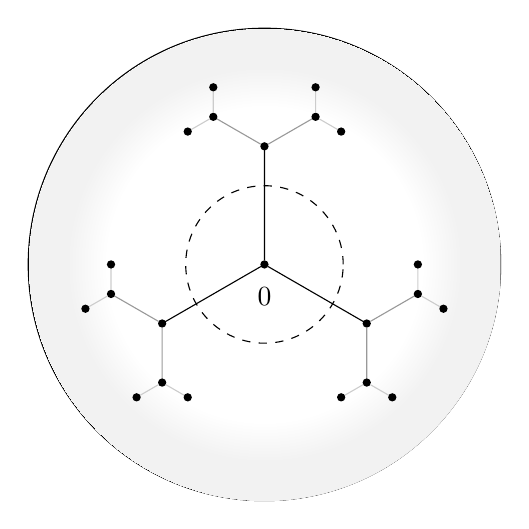
\begin{tikzpicture}[baseline=(current bounding box.center)]
% thanks to Tomasz M. Trzeciak
% based off of http://www.latex-community.org/viewtopic.php?f=4&t=2111

\draw (0,0) circle (3);

\begin{scope}
\pgfsetfading{fading3}{\pgftransformshift{\pgfpoint{0cm}{0cm}}}
\filldraw[black!5] (0,0) circle (3);
\end{scope}

\draw[dashed] (0,0) circle (1);
\coordinate[style={inner sep=0pt, outer sep=0pt, minimum size=3pt, fill=black, circle}] (O) at (0,0);
\node[below=5pt] at (O) {$0$};

\draw (O) -- +( 90:1.5) coordinate[style={inner sep=0pt, outer sep=0pt, minimum size=3pt, fill=black, circle}] (Q1)
      (O) -- +(210:1.5) coordinate[style={inner sep=0pt,outer sep=0pt,minimum size=3pt, fill=black,circle}] (Q2)
      (O) -- +(330:1.5) coordinate[style={inner sep=0pt,outer sep=0pt,minimum size=3pt, fill=black,circle}] (Q3);

\draw[black!40] (Q1) -- +(120-90:0.75) coordinate[style={inner sep=0pt, outer sep=0pt, minimum size=3pt, fill=black, circle}] (Q12)
      (Q1) -- +(240-90:0.75) coordinate[style={inner sep=0pt, outer sep=0pt, minimum size=3pt, fill=black, circle}] (Q13)
      (Q2) -- +(120-330:0.75) coordinate[style={inner sep=0pt, outer sep=0pt, minimum size=3pt, fill=black, circle}] (Q21)
      (Q2) -- +(240-330:0.75) coordinate[style={inner sep=0pt, outer sep=0pt, minimum size=3pt, fill=black, circle}] (Q23)
      (Q3) -- +(120-210:0.75) coordinate[style={inner sep=0pt, outer sep=0pt, minimum size=3pt, fill=black, circle}] (Q31)
      (Q3) -- +(240-210:0.75) coordinate[style={inner sep=0pt, outer sep=0pt, minimum size=3pt, fill=black, circle}] (Q32);

\draw[black!20] (Q12) -- +(90:0.375) coordinate[style={inner sep=0pt, outer sep=0pt, minimum size=3pt, fill=black, circle}] (Q121)
      (Q12) -- +(330:0.375) coordinate[style={inner sep=0pt, outer sep=0pt, minimum size=3pt, fill=black, circle}] (Q123)
      (Q13) -- +(90:0.375) coordinate[style={inner sep=0pt, outer sep=0pt, minimum size=3pt, fill=black, circle}] (Q131)
      (Q13) -- +(210:0.375) coordinate[style={inner sep=0pt, outer sep=0pt, minimum size=3pt, fill=black, circle}] (Q132)
      (Q21) -- +(90:0.375) coordinate[style={inner sep=0pt, outer sep=0pt, minimum size=3pt, fill=black, circle}] (Q212)
      (Q21) -- +(210:0.375) coordinate[style={inner sep=0pt, outer sep=0pt, minimum size=3pt, fill=black, circle}] (Q213)
      (Q23) -- +(210:0.375) coordinate[style={inner sep=0pt, outer sep=0pt, minimum size=3pt, fill=black, circle}] (Q231)
      (Q23) -- +(330:0.375) coordinate[style={inner sep=0pt, outer sep=0pt, minimum size=3pt, fill=black, circle}] (Q232)
      (Q31) -- +(210:0.375) coordinate[style={inner sep=0pt, outer sep=0pt, minimum size=3pt, fill=black, circle}] (Q312)
      (Q31) -- +(330:0.375) coordinate[style={inner sep=0pt, outer sep=0pt, minimum size=3pt, fill=black, circle}] (Q313)
      (Q32) -- +(90:0.375) coordinate[style={inner sep=0pt, outer sep=0pt, minimum size=3pt, fill=black, circle}] (Q321)
      (Q32) -- +(330:0.375) coordinate[style={inner sep=0pt, outer sep=0pt, minimum size=3pt, fill=black, circle}] (Q323);
\end{tikzpicture}%
%
\quad $\xrightarrow{\pi_{GH}}$ \quad%
%
\begin{tikzpicture}[baseline=(current bounding box.center)]

\newcommand\pgfmathsinandcos[3]{%
  \pgfmathsetmacro#1{sin(#3)}%
  \pgfmathsetmacro#2{cos(#3)}%
}
\newcommand\LongitudePlane[3][current plane]{%
  \pgfmathsinandcos\sinEl\cosEl{#2} % elevation
  \pgfmathsinandcos\sint\cost{#3} % azimuth
  \tikzset{#1/.style={cm={\cost,\sint*\sinEl,0,\cosEl,(0,0)}}}
}
\newcommand\DrawLongitudeCircle[2][1]{
  \LongitudePlane{35}{#2} % first argument is angle of elevation
  \tikzset{current plane/.prefix style={scale=#1}}
   % angle of "visibility"
  \pgfmathsetmacro\angVis{atan(sin(#2)*cos(35)/sin(35))} % these are angle of elevation too
  % this might assume that the angle of elevation is positive
  \draw[current plane] (\angVis:1) arc (\angVis:90:1);
  \draw[current plane,dashed] (\angVis:1) arc (\angVis:-90:1);
}

% the "2.5" magic number is the radius of the sphere 
% the "35" magic number is the angle of elevation of the camera
\pgfmathsetmacro\H{2.5*cos(35)}
\filldraw[ball color=white] (0,0) circle (2.5);
\foreach \t in {-5,-125,-245} { \DrawLongitudeCircle[2.5]{\t} }
\coordinate[style={inner sep=0pt,outer sep=0pt,minimum size=3pt,
    fill=black,circle}] (O) at (0,-\H);
\node[below=16pt] at (O) {$0$};
\coordinate[style={inner sep=0pt,outer sep=0pt,minimum size=3pt,
    fill=black,circle}] (I) at (0,\H);
\node[above=16pt] at (I) {$\infty$};
\end{tikzpicture}
\end{center}

\caption{The period map at $n = 2$, $p = 2$}
\end{figure}

\begin{theorem}\citeme{\cite{HopkinsGrossAnnouncement,StricklandGHDuality}}
\todo{Make sure you get this right.}
The sheaf $\context{E_\Gamma}(\mathbb I_{\Q/\Z})$ is the dualizing sheaf on $(\moduli{fg})^\wedge_\Gamma$. \qed
\end{theorem}





\section{Knowns and unknowns}



\subsection*{Higher orientations}

$\TAF$ and friends\label{TAFDiscussion}

The $\alpha_{1/1}$ argument: Prop 2.3.2 of Hovey's $v_n$--elements of ring spectra

% The HLP calculations

\subsection*{Equivariance}

This is tied up with the theory of power operations in a way I've never really thought about.  Seems complicated.

You should also mention the ``rigidity'' of the elliptic genus, which is about an $S^1$--equivariant version.

\subsection*{Index theorems}

Connections with analysis

The Stolz--Teichner program








-----

Bousfield's work on the $K$--theory of infinite loopspaces \cite{BousfieldLambdaRings} and Morava $K$--theoretic analogues of the results of \Cref{LEFTCooperations}
\todo{Ask Mike (and Jacob?) if there are analogues of these results for $kO$ which explain Mahowald's generalized $K$--theoretic Brown--Gitler spectra.  3/29: I did ask Mike, he said he didn't know. I also asked Paul, and he said this seemed unreasonable, since $kO$ isn't valued in co/commutative Hopf algebras.  This is a fair point: one would need to invent an ``analogue'' of Dieudonn\'e theory for $kO$, in the sense that some category it takes values in would have to be identified as abelian, where the category is rigid enough that it often sends fiber sequences to exact sequences in the category.}

Constructing sheaves of spectra on $\moduli{fg}$: the no-go results for $E_\infty$ and $A_\infty$ rings on the flat site.  There's a little MO discussion about it here: \texttt{http://chat.stackexchange.com/transcript/message/35361282\#35361282}.

Contexts for structured ring spectra

Difficulty in computing $\S_d \actson E_d^*$. (Gross--Hopkins and the period map.)

Barry's $p$--adic measures

Fixed point spectra and e.g. $L_{K(2)} \tmf$.

Blueshift, A--M--S, and the relationship to A--F--G?

Does $E_n$ receive an $E_\infty$ orientation?  Does $BP$?  (Johnson--Noel says $BP$ usually does not.  A recent preprint of Lawson says $BP$ is not even $E_\infty$ at $p = 2$!!!)

$p$--divisible groups and transchromatic phenomena

Remark 12.13 of published $H_\infty$ AHS says their obstruction framework agrees with the $E_\infty$ obstruction framework (if you take everything in sight to have $E_\infty$ structures).  This is almost certainly related to the discussion at the end of Matt's thesis about the $MU$--orientation of $E_d$.\todo{Section 12.4 compares doing $H_\infty$ descent with doing $E_\infty$ descent and shows that they're the same (in the case of interest?).}

Hovey's paper on $v_n$--periodic elements in ring spectra.  He has a nice (and thorough!) exposition on why one should be interested in bordism spectra and their splittings: for instance, a careful analysis of $M\Spin$ will inexorably lead one toward studying $KO$.  It would be nice if studying $M\String$ (and potentially higher analogues) would lead one toward non-completed, non-connective versions of $EO_n$.  Talk about $BoP$, for instance.

Matt's short resolutions of chromatically localized $MU$.

Nilpotency and vanishing curves in the ($MU$--)Adams spectral sequence.  The \emph{non}-nilpotency of $\eta$ in the $MU$--Adams spectral sequence.  Mathew--Meier type theorems about horizontal vanishing lines and the Tate construction (and related results about the $\TMF$ spectral sequence and the Johnson--Wilson theories).

Additive degeneration and $kO \ne kU^{hC_2}$.






\begin{remark}
It is completely unclear why $MU$ plays such an important mediating role between geometry (i.e., the stable category) and algebra (i.e., sheaves on the moduli of formal groups).  Given a general ring spectrum $R$ and thick prime $\otimes$--ideals $\CatOf C_\alpha$ of perfect $R$--modules, one ask the analogous two questions:
\begin{enumerate}
\item Is it possible to find an $R$--algebra $S$ whose context functor induces a homeomorphism of Balmer spectra $\Spec(\CatOf{Modules}_R^{\perf}) \to \Spec(\CatOf{QCoh}(\context{S/R}))$?
\item Are there complementary localizers $L_\alpha\co \CatOf{Modules}_R \to \CatOf{Modules}_{R,(\alpha)}$?  Can they be presented via Bousfield's framework as homological localizations for auxiliary $S$--algebra spectra $S_\alpha$?  Do the contexts $\context{S_\alpha}$ admit compatible localizers with $\context{S}$?
\end{enumerate}
For $R = \S$, this is the role that the $R$--algebra $S = MU$ and the $S$--algebras $S_d = E(d)$ play.  Finding these spectra feels like striking gold, and it is unclear how to produce analogous spectra in general.
\todo{Mathews's work on Galois descent shows that the fixed point map $\CatOf{Modules}_{E_\Gamma, \Aut \Gamma}^{\mathrm{complete}} \to \CatOf{Spectra}_{\Gamma}$ is an equivalence of categories.}
\end{remark}
\noindent One can ask the same question from the geometric direction: why bordism?  Why should these spectra have these nice flatness properties?  Why should they have recognizable computational properties?  Why bordism?




\begin{remark}
The homotopy of $\widehat L_2 \S$ is also known, by work of Shimomura and collaborators~\cite{Shimomura,ShimomuraYabeM20,ShimomuraYabeL2S} (but see also the reorganization by Behrens~\cite{BehrensRevisited}).  It is \emph{exceedingly} complicated, and it is an open problem to find an expression of it which admits human digestion.  Behrens has pursued a program encoding this problem in terms of modular forms~\cite{BehrensCongruences,BehrensModularDescription,BehrensBuildings}, and Hopkins has proposed a program involving $L$--functions~\cite{StricklandpAdicInterpolation}, motivated by which Hovey and Strickland have shown a kind of continuity result for among the groups~\cite[Section 14]{HoveyStrickland}.
\end{remark}





\begin{remark}
There are also ``finitary'' flavors of chromatic localization available, which are typically less robust but more computable.  They assemble into a diagram:
\begin{center}
\begin{tikzcd}
E \arrow{r} \arrow{d} & L_d^{\fin} E \arrow{r} \arrow{d} & L_d E \arrow{d} \\
L_{X(d)} E \arrow{r} & \widehat L_d^{\fin} E \arrow{r} & \widehat L_d E,
\end{tikzcd}
\end{center}
where $X(d)$ is a finite complex of type exactly $d$, $v$ is a $v_d$--self-map of $X(d)$, $T(d) = X(d)[v^{-1}]$ is the localizing telescope, $\widehat L_d^{\fin}$ is Bousfield localization with respect to $T(d)$ (which can be shown to be independent of choice of $X(d)$ and of $v$), and $L_d^{\fin}$ denotes localization with respect to the class of \emph{finite} $E(d)$--acyclics.  Many things about these functors are known: for instance, $L_{X(d)} L_d = \widehat L_d$, there is a chromatic fracture square relating $L_d^{\fin}$ to $\widehat L_{\le d}^{\fin}$, and $L_d^{\fin} E \simeq L_d E$ if and only if $\widehat L_{\le d}^{\fin} E \simeq \widehat L_{\le d} E$.  One major question about these functors remains open, corresponding the last unsettled nilpotence and periodicity conjecture of Ravenel~\cite[Conjecture 10.5]{RavenelLocalizationWRTPeriodic}: is the map $\widehat L_d^{\fin} E \to \widehat L_d E$ an equivalence?  Multiple proofs and disproofs have been offered, but the literature remains unsettled.
\citeme{Find some proofs and disproofs.}
\end{remark}







\begin{remark}
Writing $M_d$ for the fiber in the sequence $M_d \to L_d \to L_{d-1}$, the filtration spectral sequence associated to the tower in \Cref{ChromaticConvergence} is called the \textit{geometric chromatic spectral sequence}, which has the form $\pi_* M_* \S \Rightarrow \pi_* \S_{(p)}$.  The two forms of filtration data $M_d X$ and $\widehat L_d X$ are actually functorially equivalent to one another:
\begin{align*}
\widehat L_d M_d & \simeq \widehat L_d, &
M_d \widehat L_d & \simeq M_d,
\end{align*}
but they have fairly distinct properties.  For instance, $M_d$ is smashing whereas $\widehat L_d$ is not, $M_d$ is not part of an adjoint pair whereas $\widehat L_d$ is, and the analogue of \Cref{FormulaForKnLocalization} for $M_d$ is ``backwards'':\citeme{I forget who this is due to} \[M_d X \simeq \colim_I \left( M^0(v^I) \sm L_d X \right).\]  The spectrum $M_d X$ also relates to the chromatic fracture square for $X$:
\begin{center}
\begin{tikzcd}
M_d X \arrow{d} \arrow[equal]{r} & M_d X \arrow{d} \\
L_d X \arrow{r} \arrow{d} \arrow[dr, phantom, "\lrcorner", very near start] & \widehat L_d X \arrow{d} \\
L_{d-1} X \arrow{r} & L_{d-1} \widehat L_d X.
\end{tikzcd}
\end{center}
From this, we see that there is a fiber sequence $M_d X \to \widehat L_d X \to L_{d-1} \widehat L_d X$.

The case $d = 1$ gives the prototypical example of the difference between these two presentations of the ``exact height $d$ data'', where the sequence becomes: \[\colim_j (M^0(p^j) \sm L_1 X) \to \lim_j (M_0(p^j) \sm L_1 X) \to \left( \lim_j (M_0(p^j) \sm L_1 X) \right)_{\Q}.\]  If, for instance, $\pi_0 L_1 X = \Z_{(p)}$, then the long exact sequence of homotopy groups associated to this fiber sequence gives
\begin{center}
\begin{tikzcd}
\pi_0 \widehat L_1 X \arrow{r} \arrow[equal]{d} & \pi_0 L_0 \widehat L_1 X \arrow{r} \arrow[equal]{d} & \pi_{-1} M_1 X \arrow[equal]{d} \\
\Z^\wedge_p \arrow{r} & \Q_p \arrow{r} & \Z/p^\infty.
\end{tikzcd}
\end{center}
Coupling this to \Cref{piLK1SExample}, we compute
\begin{align*}
\pi_t M_1 \S^0 & = \begin{cases} \Z/p^\infty & \text{when $t = -1$}, \\ \Z_p / (pk) & \text{when $t = k|v_1| - 1$ and $t = \ne 0$}, \\ \Z/p^\infty & \text{when $t = (0 \cdot |v_1| - 1) - 1 = -2$}, \\ 0 & \text{otherwise}. \end{cases}
\end{align*}
This is a model for what happens generally when passing from $\pi_* \widehat L_d X$ to $\pi_* M_d X$: the $v_j$--torsion--free groups get converted to infinitely $v_j$--divisible groups, with some dimension shifts.\footnote{A height $2$ example of this same phenomenon is visible in Behrens's paper~\cite[Section 7]{BehrensRevisited}.}
\end{remark}




\begin{theorem}[Unpublished work of Hopkins and Lurie]
Let $F_d$ denote the discrepancy spectrum for $E_d$.  There is a natural equivalence of infinite loopspaces $\Loops^\infty F_d \simeq \Susp^d \mathbb I_{\Q/\Z}$. \qed
\end{theorem}




free $E_\infty$--orientations off of $MU$






Sections 5.3-4 of Hopkins's ICM address \textit{Algebraic Topology and Modular Forms} has a discussion of what $\eta$ and $\nu$ have to do with $\tmf$, as well as the construction of some interesting ``topological $\theta$--series'' in the elliptic cohomology of certain Thom complexes.



\todo[inline]{Jacob wrote me an email giving a very slightly fuller sketch of what the DAG perspective on the $\sigma$--orientation is.  Interestingly, it boils down to a fact from projective geometry: there just aren't that many line bundles on projective varieties.  This forces a couple of things to become equal, and in a suitable setting they even become canonically equal.  The email has no subject line, which will make it hard to find, but you should include a summary of it (which is dependent on whatever's written in the \textit{Survey} paper) all the same.}



